
\chapter{协议实现}

本周修改的主要是 liso\_server 的接收请求部分的代码。在 while(1) 的服务器处理循环中添加以 select 开头的预处理等操作,使服务器能够在等待一个客户端发送下一个请求时,同时处理来自其他客户端的请求,使服务器能够同时处理多个并发的客户端。

\section{处理并发客户端的实现}


\paragraph*{}

大体逻辑如下图\ref{fig:flowchar}所示。因空间限制,未完全采用规范画法。
%%% 添加流程图

\begin{figure}[htbp!]
    \centering
    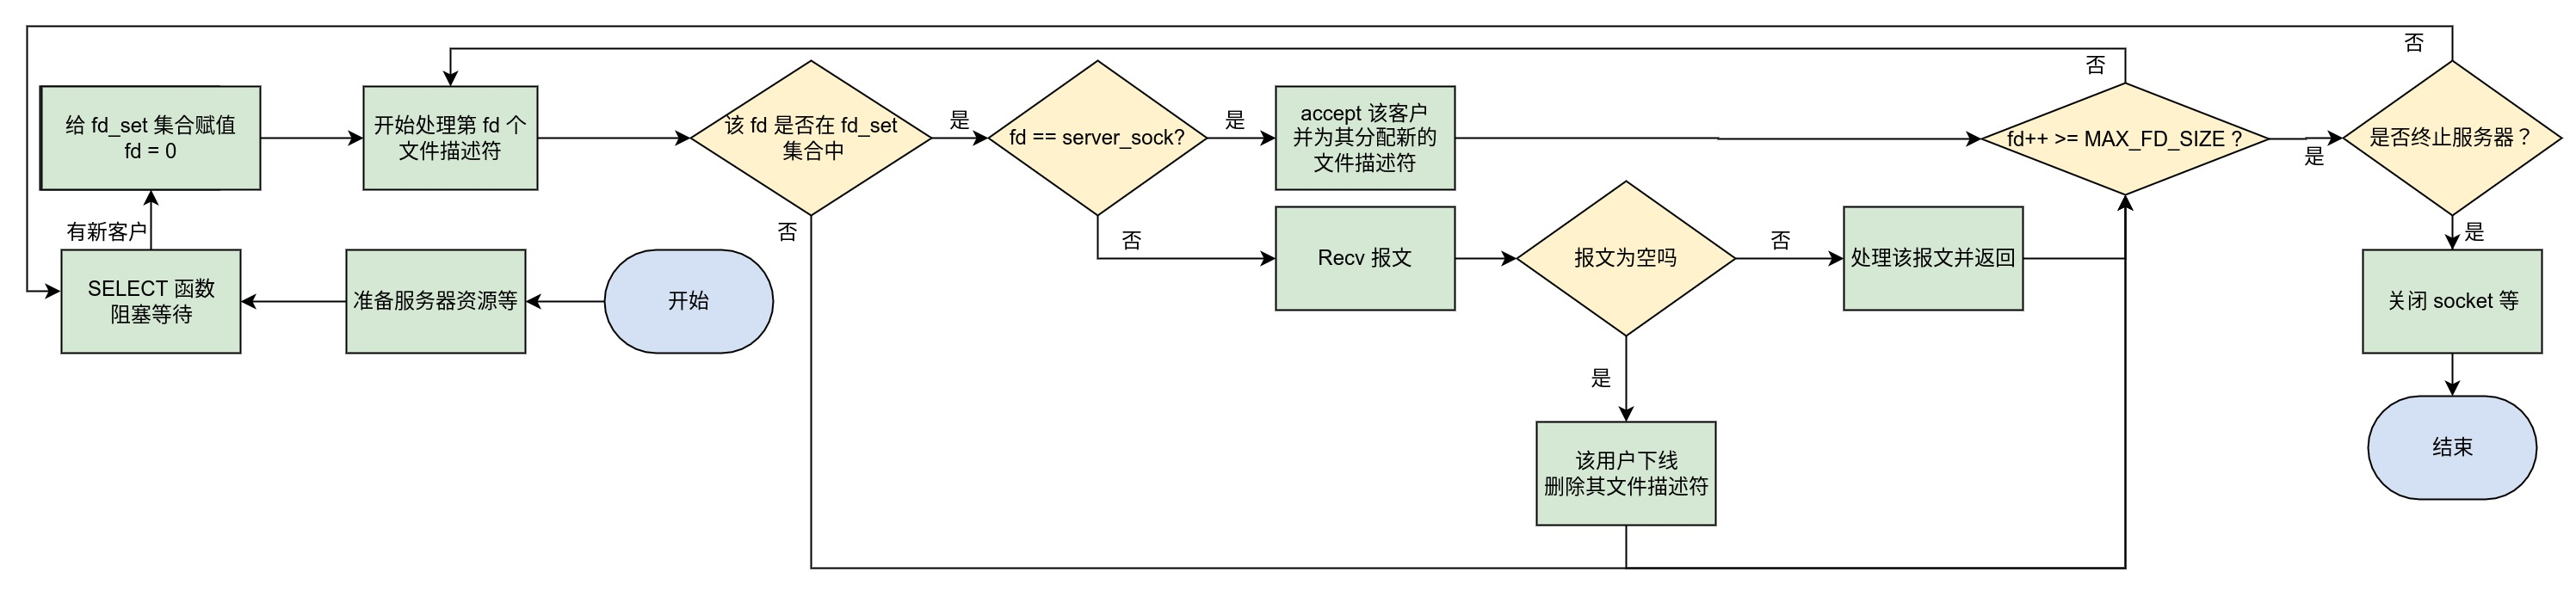
\includegraphics[width=6in]{FlowChart.jpg}
    \caption{流程图}\label{fig:flowchar}
\end{figure}


首先使用 cnt=select(MAX\_FD\_SIZE+1, \&tmp\_fds, NULL, NULL, NULL) 获取当前总共有多少个客户端有请求,同时将他们的文件描述符添加到类型为 fd\_set 的集合中,将用户总数返回给 cnt 变量。

然后循环遍历 fd\_set 集合中 0~MAX\_FD\_SIZE 个位置。通过函数 FD\_ISSET() 判断当前位是否有客户。如果有客户占用,则进行处理,否则跳过。

在处理时,先判断其文件描述符是否和服务器的 sock 相同,如果相同则表明是一个新的连接,需要进行 accept 操作,并为其分配一个新的文件描述符。如果和服务器的 sock 不相同,则按照一般流程处理。如果使用 select 选择了这个客户,且后续 recv 函数接收到的信息长度为 0,我们就可以认为这个客户已经离去,可以关掉它的 socket 了。

和前几次的一个小区别在于服务器需要为每个客户分配一个私有的空间来存储它的地址、端口以及缓存。对此,我们的实现方式,是使用地址类型和动态伸缩的数组。(也可以使用结构体,不过原理是一样的)。


